\documentclass[a4paper, 12pt]{article}
\usepackage[a4paper, left=30mm, right=30mm, top=30mm, bottom=30mm, marginpar=25mm]{geometry}
\usepackage{indentfirst}
\usepackage{float}
\usepackage{graphicx}
\usepackage{amsmath}
\usepackage{amsfonts}
\usepackage{amssymb}
\usepackage{geometry}
\usepackage{listings}
\usepackage{xcolor}
\usepackage{fancyhdr}
\usepackage{lastpage}
\pagestyle{fancy}
\setlength{\headheight}{29.5pt}
\definecolor{codegreen}{rgb}{0,0.6,0}
\definecolor{codegray}{rgb}{0.5,0.5,0.5}
\definecolor{codepurple}{rgb}{0.58,0,0.82}
\definecolor{backcolour}{rgb}{0.95,0.95,0.92}
\lstset{
    backgroundcolor=\color{backcolour},   
    commentstyle=\color{codegreen},
    keywordstyle=\color{blue},
    numberstyle=\tiny\color{codegray},
    stringstyle=\color{codepurple},
    basicstyle=\ttfamily\footnotesize,
    breakatwhitespace=false,         
    breaklines=true,                 
    captionpos=b,                    
    keepspaces=true,                 
    numbers=left,                    
    numbersep=5pt,                  
    showspaces=false,                
    showstringspaces=false,
    showtabs=false,                  
    tabsize=2
}

\renewcommand{\contentsname}{Índice}

\renewcommand*{\maketitle}{
\thispagestyle{plain}
\begin{center}
    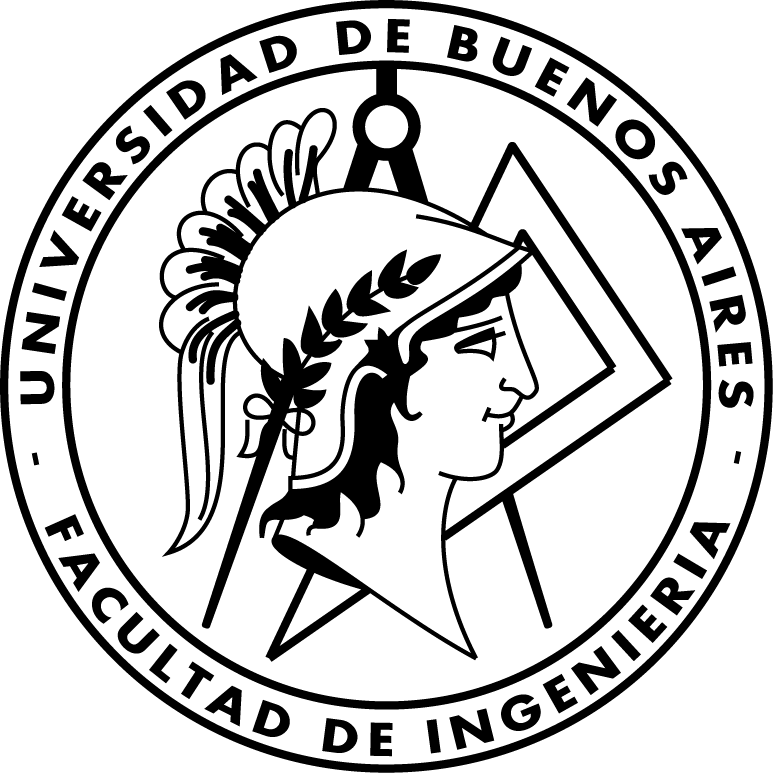
\includegraphics[width=7cm]{Logo-fiuba.png} 
    \\[1cm]
    \textsc{\Large Teoría de Algoritmos}\\           
    \textsc{\small Curso Echevarria}\\[0.4cm]    
    { \huge \bfseries Trabajo Práctico 1 }\\[0.3cm]      
    \rule{\textwidth}{0.4pt} \\[0.2cm] 
    {\large \today  \\[0.4cm]}                          
    \begin{minipage}{0.4\textwidth}
    \begin{flushleft}
        \large{
        \begin{itemize}
            \item Juan Claros - 111254
            \item Yoel Gaston Arlia - 111520
            \item Guido Cuppari - 111172
            \item Josue Daniel Mamani - 111514
        \end{itemize}
        }
    \end{flushleft}
\end{minipage}

\end{center}
}

\title{x}

\begin{document}

\maketitle

\newpage

\tableofcontents

\newpage
\section{Problema 1}
\subsection{Supuestos}
\begin{itemize}
    \item Se supone que las cargas estan almacenadas en una lista Q, de manera equidistante y cada posicion de la lista representa la posicion de las particulas
\end{itemize}
\subsection{Diseño}
\begin{itemize}
    \item En el main, se generan los archivos que almacenan las cargas, donde cada posicion tiene un valor de carga ditinta, desde -10 hasta 10.
    \item La funcion calcular fuerza aplica un algoritmo de Division y Conquista, dividiendo el problema en subproblemas y juntando los resultados. El arreglo de cargas Q se divide recursivamente en mitades hasta llegar a subconjuntos de tamaño 1. Después de calcular las fuerzas dentro de cada mitad, se computan las interacciones cruzadas entre las partículas de la mitad izquierda y la mitad derecha. Esto asegura que todas las combinaciones (i, j) con i < j sean consideradas exactamente una vez. Las fuerzas se acumulan: F[i] recibe una fuerza negativa (j lo repele o atrae) y F[j] una positiva (i lo repele o atrae).


\end{itemize}

\subsection{Analisis de Complejidad}
\begin{itemize}
    \item La declaracion de variables es O(1), la division en subproblemas recursivamente es O(log n), luego con los dos for anidados se trata de, en el peor de los casos, \(O(N^2)\). 
\end{itemize}
\subsection{Seguimiento}
\begin{itemize}
    \item Se toma como ejemplo el vector de cargas \( q = [2, -1, 3, 1] \). El algoritmo comienza inicializando un arreglo de fuerzas \( F \) con ceros. Luego, se aplica recursivamente la estrategia de división y conquista, dividiendo el vector en mitades, resolviendo internamente cada una y luego calculando las interacciones cruzadas entre las mitades.

    \item En este caso, se procesan las interacciones entre las partículas de la izquierda (\([2, -1]\)) y las de la derecha (\([3, 1]\)), actualizando la fuerza neta sobre cada partícula según la ley de Coulomb simplificada: \( F = C \cdot \frac{q_i \cdot q_j}{d^2} \), donde \( d \) es la distancia entre partículas. Al finalizar, el vector de fuerzas contiene los valores netos acumulados para cada partícula: \( F = [-1.722, 3.25, -1.5, -0.028] \), que representa la fuerza total que recibe cada carga del sistema.

\end{itemize}
\subsection{Mediciones}
\begin{figure}[h]
		\centering
		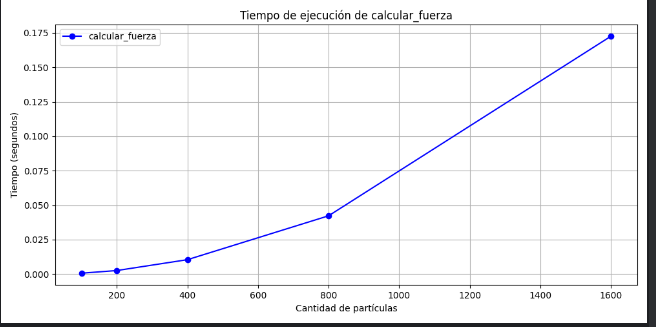
\includegraphics[width=\textwidth]{ej1.png}
	\end{figure}
\subsection{Resultados}
\begin{itemize}
    \item Los resultados, segun la medicion realizada, son los esperados a partir del analisis realizados previamente
\end{itemize}
\subsection{Generacion de sets}
\begin{itemize}
    \item Los sets son realizados a partir de una funcion randomizada, que generan archivos de texto con listas que representan las cargas a probar.
\end{itemize}

\section{Problema 2}

\subsection{Supuestos}

\begin{itemize}
	\item Se supone que las distancias se encuentran en una lista, donde cada posición es la distancia a la anterior posición, y cada posición representa una parada. El resultado se genera almacenando los subíndices de cada parada.
\end{itemize}

\subsection{Diseño}

\begin{itemize}
    \item En el main, se generan los archivos que almacenan las distancias a evaluar con una semilla fija, luego se generan los archivos donde van los resultados y se llama a la funcion que realiza el calculo.
    \item La funcion generar\_datos, genera una lista con datos aleatorios basandose en la semilla recibida, estos datos son numeros enteros de 0 a 7 inclusive y se genera una lista de largo recibido que es retornada.
    \item La funcion calcular\_mejor\_distancia recorre mientras que el elemento que estoy evaluando es menor que el largo de la lista de paradas, y luego avanza mientras que la suma de distancias sea menor que 7, modificando la posicion actual y luego una vez que la suma exceda 7 se agrega a la lista de resultados el indice -1 que seria la posicion que cumple el rango, luego continua siguiendo esta misma idea, y agrega el ultimo paraje para llegar hasta el final, imprime el tiempo que tardo y devuelve una lista con los resultados.
    
\end{itemize}

\subsection{Analisis de complejidad}

\begin{itemize}
    \item La parte de generar los datos no la tengo en cuenta en el analisis, solo la parte de calcular los resultados, time es O(1), inicializar variables tambien es O(1), len(distancias), es O(1), imprimir y utilizar append es O(1), los while anidados, comparten la condicion de que la posicion sea menor que el largo y en cada iteracion se avanza al menos una vez, por lo que la complejidad de esta parte es O(n), como conclusion, el resultado es O(n).

\end{itemize}

\subsection{Seguimiento de Ejemplo}
\begin{itemize}
    \item Vamos a hacer un ejemplo con la lista de distancias = [4, 3, 6, 6, 1, 7], Al llegar a la funcion se inicializan las variables, y el largo queda en 5, se entra al primer while ya que i esta en 0 que es menor que el largo, luego se entra al otro while, repitiendo la condicion y evaluando que el elemento en la lista en la posicion i (0) sea menor o igual que 7, como es el caso (4), se entra al while y se suma el actual en auxiliar(4) y se aumenta la posicion(1), como ahora la posicion es 1 y la suma en auxiliar es 4, evaluando la condicion en auxiliar + el valor en la nueva posicion(1) (valor = 3), como auxiliar(7) es menor o igual que 7, se suma este  valor parcial en auxiliar(7) y se suma en 1 la posicion(2), ahora al evaluar la condicion de menor o igual que 7 va a dar false porque el valor es 13 que es mayor, se sale de este while, se guarda el indice de la posicion actual a la anterior (2-1), y se continua iterando de esta forma hasta llegar a la ultima posicion (5), donde esta posicion ya no es menor que el largo por lo que se deja de iterar y se agrega este indice, se calcula e imprime el tiempo final. Devuelve una lista con los resultados obtenidos.
\end{itemize}


\subsection{Casos de prueba y mediciones}


    \begin{figure}[h]
		\centering
		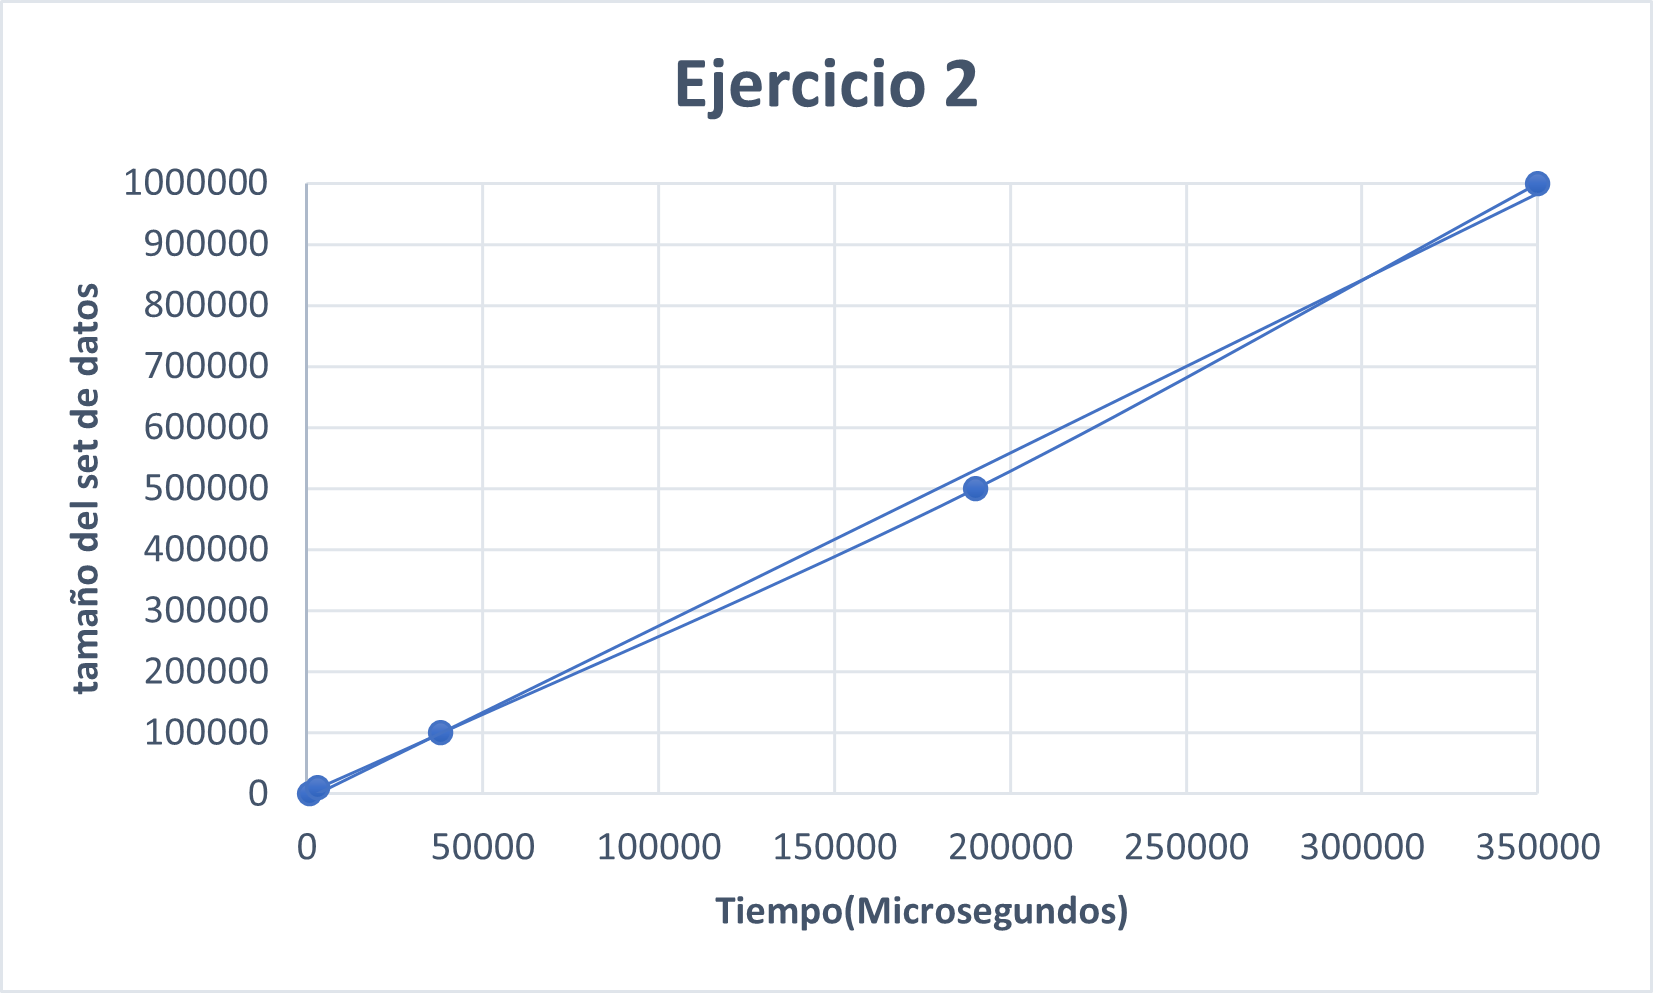
\includegraphics[width=\textwidth]{ej2.png}
	\end{figure}

\subsection{Resultados}
\begin{itemize}
    \item Los resultados para 1000, 10000, 100000, 500000 y 1000000, son lo esperado 
     y coincide con la complejidad analizada O(n).
\end{itemize}

\subsection{Referencias}

\begin{itemize}
    \item Van Rossum, G., \& Python Software Foundation. (2023). Built-in Functions: open. Retrieved from https://docs.python.org/3/library/functions.html\#open
    \item Sedgewick, R., \& Wayne, K. (2011). Algorithms (4th ed.). Addison-Wesley.
\end{itemize}

\subsection{Generacion de sets}
\begin{itemize}
\item para generar los sets se realiza de la siguiente manera, utilizando 1 como semilla para el largo 1000, 2 como semilla para el largo 100000, 3, como semilla para largo 100000, 4 como semilla para largo 500000, y 5 como semilla para largo 1000000.

    \begin{lstlisting}[frame=single]
    def generar_datos(largo, semilla):
    random.seed(semilla)
    return [random.randint(0, MAXIMA_DISTANCIA) for _ in range(largo)]
\end{lstlisting}
\end{itemize}

\section{Problema 3}

\subsection{Enunciado y supuestos}

Una suma encadenada es una secuencia de números a0, a1, ..., an tal que a0=1 y para cada k>0: ak=ai+aj para algún i, j, k. Por ejemplo, 1, 2, 3, 6 es una suma encadenada para 6 de longitud 3 ya que:

\begin{itemize}
	\item 2=1+1
	\item 3=2+1
	\item 6=3+3
\end{itemize}

\indent Para desarrollar un algoritmo de Backtracking que pueda calcular una suma encadenada de longitud mínima para un entero positivo n y tambien tiene que ser n >= 2 ya que no tiene sentido calcular un n = 1 ya que es sencillo.

\subsection{Diseño}
Para este ejercicio, se utilizo bactraking el cual se implemento utilizando la recursivida, se penso en un arbol que contenga las posibles soluciones para un n buscado siendo la raiz 1 y siendo los hijos las posibles sumas encadenas posibles por las sumas de los nodos  rrecoridos desde la raiz haste un hijo dado, el recorrido del la raiz hasta el hijo seria la longitud de la suma encadenada. La manera de recorrer el arbol es meramente parecida a DFS.
    por ejemplo tenemos como recorrido inicial a recorrido = [1] las posibles sumas encadenadas posibloes son 2  = 1 + 1 y leugo 2 tiene dos posibles hijos que serian 4 = 2 + 2 y 3 = 3 + 1 perel algoritmos va recorriendo el arbol de derecha a esquierda y asi iterando suma por suma terminamos recorriendo todo;

\subsection{Pseudocodigo}
	\begin{lstlisting}[frame=single]
		bactraking(camino, objetivo, inicio, resultado, suma)
			#caso base
			si suma = objetivo
				si len(resultado) == 1 and len(resultado[0]) > len(recorrido)
					resultado = recorrido
				si len(resultado) == 0:
					resultado = recorrido
				return
			#corte o poda
			si suma > n or len(resultado) != 0 and len(recorrido) > len(resultado[0]):
				return
			indice = len(recorrido) - 1
			#recorriendo las posibles soluciones
			siempre que len(recorrido) >= 1 and indice <= len(recorrido) - 1 and indice >= 0
				longitud = len(recorrido) - 1
				si es la primera iteracion entonces
					suma = recorrido[indice] + recorrido[longitud]
					a recorrido agregar suma
					backtracking(recorrido,n,len(recorrido) - 1,resultado,suma)
					return resultado
				sino
					suma = recorrido[indice] + recorrido[longitud]
					a recorrido agregar suma
					si indice > 0
						backtracking(recorrido,n,len(recorrido) - 1,resultado,suma)
					else: 
						backtracking(recorrido,n,indice,resultado,suma)                   
						eliminar el ultimo elemento de rrecorrido
					indice = indice - 1	
			
	\end{lstlisting}


\subsection{Seguimiento}

    \begin{figure}[h]
		\centering
		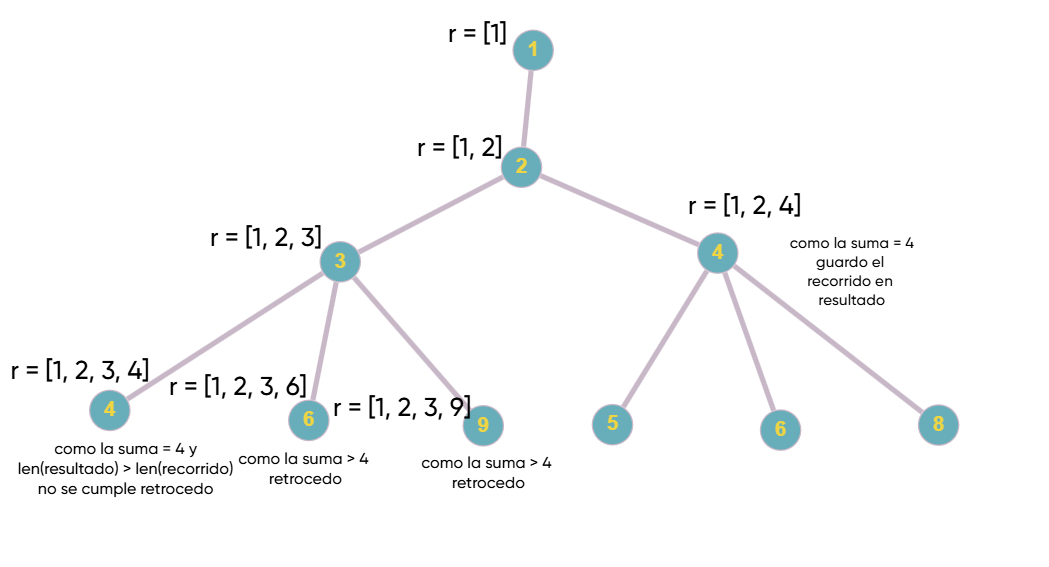
\includegraphics[width=\textwidth]{arbol.jpg}
	\end{figure}

Para el seguimiento tomamos como n = 4 para encontrar la menor suma encadenada dando como resultado una longitud de 2 los cuales serian 2 = 1 + 1 y 4 = 2 + 2, que se vera mas claro como seria el seguimiento para encontrar en la imagen siguiente.
    
	

\subsection{Complejidad}
	
	
	El algoritmo que implementa bactraking explora todas las posibles sumas encadenadas que se pueden hacer con los elementos de un estado de rrecorrido, por ejemplo si recorrido = [1, 2, 4] las posibles sumas encadenas son 
\begin{itemize}
	\item  \(5 = 1 + 4\)
	\item \(6 = 4 + 2\)
	\item \(8 = 4 + 4\)
\end{itemize}
    cada una de estas combinaciones posibles genera una nueva llamada recursiva, por lo tanto cada llamada recursiva puede tener multiples hijos el cual va en aument0 si el n esmayor y a medida que la variables rrecorido va en aumento tambien aumentario los hijos generados de mane exponecial en el peor de los caso, por lo tanto la complejidad en el peor  de los caso es O(2^n)

	
\subsection{Set de datos}
los sed de datos para el problema se generan de con el siguiente codigo 
	\begin{lstlisting}[frame=single]
		def generar_sets(cantidad, semilla=42):
		random.seed(semilla)
		sets = []
		for _ in range(cantidad):
			n = random.randint(5, 200)
			sets.append(n)
		return sets	
	\end{lstlisting}
	
\subsection{Tiempos de ejecución}

	\begin{figure}[H]
		\centering
		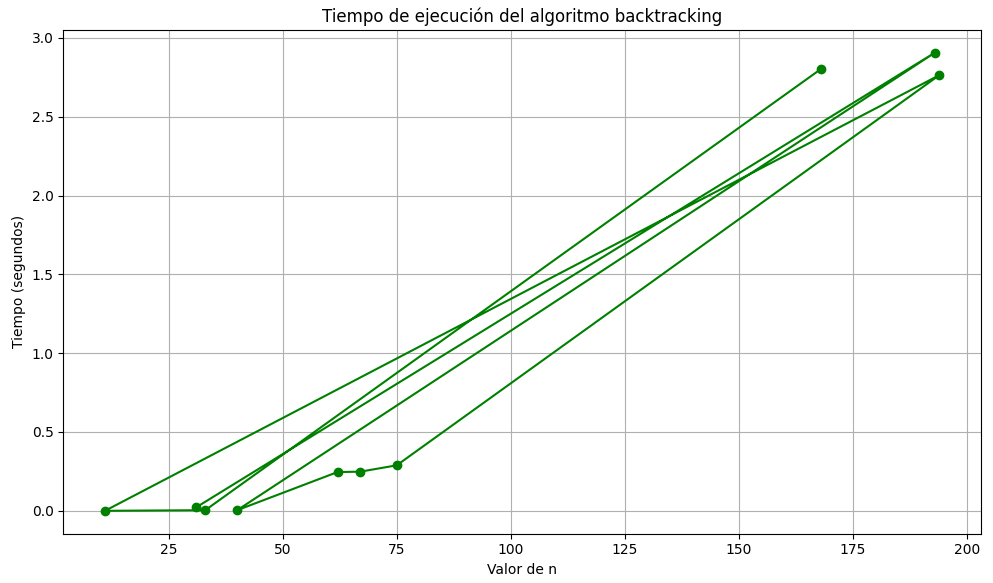
\includegraphics[width=\textwidth]{grafico.png}
	\end{figure}
    

\subsection{Informe de resultados}

    Por medio del grafico corresponde como \(O(2^n)\) en el peor de los casos que seria que se hagan todas las posibles sumas encadenas, en le grafico vemos que al pricipio los valores de n como por ejemplo entre n = 0 hasta n = 50 el tiempo es casi 0 pero despues con valor aprox 150 se eleva exponencialmente y los demas valores, el cual es un compotamiento de la complejidad exponencial, tambien pueden haber valores de n que podriamos pensar que su tiempo aumentaria exponencialmente pero tambien puede que tarde menos de los pensado ya que el algoritmo puede tambien podar y eso causaria que tarde menos y eso reduciria su tiempo.
    
    
    
\end{document}